\documentclass[tikz,border=10pt]{standalone}
\usepackage{amsmath}
\usepackage{amssymb}
\usepackage{tikz}
\usetikzlibrary{arrows.meta,calc}

\definecolor{figazul}{RGB}{2,132,199}
\definecolor{figrojo}{RGB}{220,38,38}
\definecolor{figverde}{RGB}{22,163,74}

\begin{document}
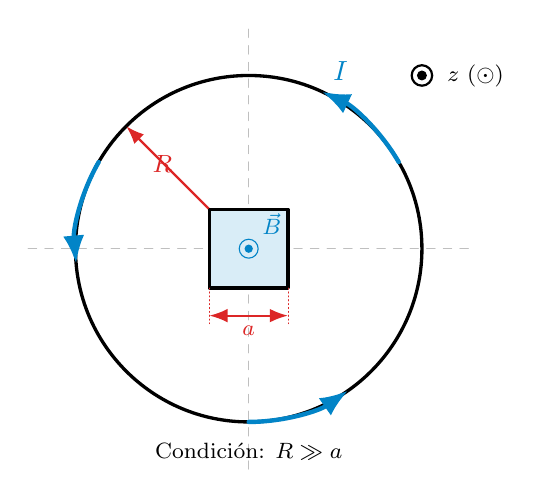
\begin{tikzpicture}[>=Latex, line cap=round, line join=round]
  % Ejes tenues de referencia
  \draw[dashed, color=gray!50] (-2.8, 0) -- (2.8, 0);
  \draw[dashed, color=gray!50] (0, -2.8) -- (0, 2.8);

  % Espira circular grande de radio R
  \draw[very thick] (0, 0) circle (2.2);

  % Flechas de corriente I en sentido antihorario
  \draw[->, ultra thick, color=figazul] (30:2.2) arc (30:65:2.2) node[above right, color=figazul] {$I$};
  \draw[->, ultra thick, color=figazul] (150:2.2) arc (150:185:2.2);
  \draw[->, ultra thick, color=figazul] (270:2.2) arc (270:305:2.2);

  % Cota del radio R (en rojo)
  \draw[->, thick, color=figrojo] (0, 0) -- (135:2.2);
  \node[above left, color=figrojo, font=\small] at (135:1.2) {$R$};

  % Espira cuadrada concéntrica de lado a (a << R)
  \draw[very thick, fill=figazul!15] (-0.5, -0.5) rectangle (0.5, 0.5);

  % Campo B producido en el centro (puntos \odot salientes en azul)
  \draw[thin, color=figazul] (0, 0) circle (0.12);
  \fill[color=figazul] (0, 0) circle (1.5pt);
  \node[above right, font=\footnotesize, color=figazul] at (0.05, 0.05) {$\vec{B}$};

  % Cota del lado a de la espira cuadrada (en rojo)
  \draw[<->, thick, color=figrojo] (-0.5, -0.85) -- (0.5, -0.85) node[midway, below, color=figrojo, font=\footnotesize] {$a$};
  \draw[densely dotted, thin, color=figrojo] (-0.5, -0.5) -- (-0.5, -0.95);
  \draw[densely dotted, thin, color=figrojo] (0.5, -0.5) -- (0.5, -0.95);

  % Eje z saliente a un costado
  \draw[thick] (2.2, 2.2) circle (0.13);
  \fill (2.2, 2.2) circle (1.8pt);
  \node[right, font=\footnotesize] at (2.4, 2.2) {$z$ ($\odot$)};

  % Condición R >> a
  \node[below, font=\footnotesize] at (0, -2.35) {Condici\'on: $R \gg a$};
\end{tikzpicture}
\end{document}
